\documentclass{article}
\usepackage{amsmath}
\usepackage{amssymb}
\usepackage{graphicx}
\usepackage{hyperref}
\usepackage[version=4]{mhchem}


\begin{document}
\(D A\) and \(D B\) are tangent to circle \(O\) at \(A\) and \(B\), respectively. \(A C\) is the diameter of circle \(O\). Prove: \(\angle A D B=2 \angle B A C\).

Solution:
Connect \(O B\).\\
Since both \(O A\) and \(O B\) are radius, \(O A=O B\) and \(\angle O A B\)\\
\centering
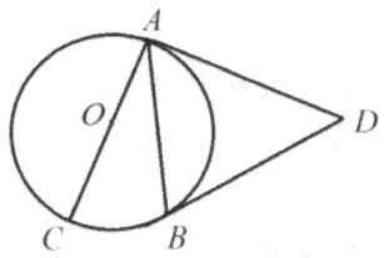
\includegraphics[width=\textwidth]{images/147.jpg}\\
\(=\angle O B A=\alpha\).\\
Since \(\angle C O B\) is the exterior angle of triangle \(A B O\),\\
\(\angle C O B=\beta=2 \alpha\).\\
In quadrilateral \(A D B O, \angle A D B+\angle D B O+\angle B O A+\) \(\angle O A D=360^{\circ} \Rightarrow \quad \angle A D B+90^{\circ}+\angle B O A+90^{\circ}=\) \(360^{\circ}\)\\
\centering
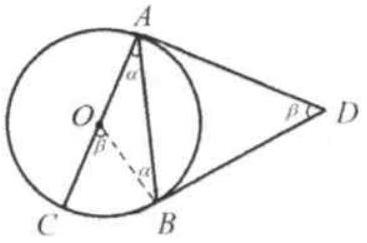
\includegraphics[width=\textwidth]{images/147(3).jpg}\\
\(\Rightarrow \quad \angle A D B+\angle B O A=180^{\circ}\)\\
Since \(\angle B O A=180^{\circ}-\beta\), (1) becomes \(\angle A D B+180^{\circ}-\beta=180^{\circ}\)\\
\(\Rightarrow \quad \angle A D B=\beta=2 \alpha\).\\
That is, \(\angle A D B=2 \angle B A C\).



\end{document}
